% abstract 
\begin{abstract}
\sloppy
  This thesis proposes the design and implementation of a 
    high-performance 
      simulation sandbox for developing and testing decentralized control 
      algorithms for autonomous sailing drone swarms. 
      The core of the project is a simulation environment.
      The simulator models key marine dynamics, including wind and sea conditions, 
      and incorporates virtual sensors, 
      along with inter-drone communication channels.

      \vspace{1em}

      The motivation for this work is its application in maritime search and rescue (SAR).
      By leveraging a swarm of inexpensive, autonomous drones, the 
      time to locate a drowning victim can be significantly reduced, dramatically 
      increasing the chances of survival. 

      \vspace{1em}

      As of October 2025, there are no known existing solutions that combine simulation,
      SITL/HITL capabilities, and decentralized control for marine drone swarms,
      making this project a pioneering effort in autonomous maritime robotics.
      Existing tools tend to target aerial drones or are general-purpose robotics
      simulators and require heavy modification to support marine dynamics and
      large-scale swarm experiments. A related project is YARA\cite{YARA}, a
      Gazebo-based sailing drone simulator, but it lacks SITL/HITL support and is
      not optimized for extensive swarm simulations.

      \vspace{1em}

      This work will implement a cross-robot communication channel model with
      signal attenuation, delays, and packet dropouts. The simulator will provide
      sensor models for IMU, GPS, and AIS (Automatic Identification System) 
      and will support replaying historical AIS datasets to
      populate and simulate real vessel traffic within the environment. The
      platform will also allow isolating and instantiating independent swarms
      to enable large-scale training and
      evaluation of genetic algorithms and neural-network based controllers.
      \vspace{1em}

      The simulator will be validated through a series of experiments, including
      benchmarking decentralized control algorithms for formation keeping,
      collision avoidance, and cooperative search tasks. The performance of the
      simulator will be assessed based on its computational efficiency, scalability,
      and fidelity in replicating real-world marine conditions.

      \vspace{0.4em}
      \begin{center}
        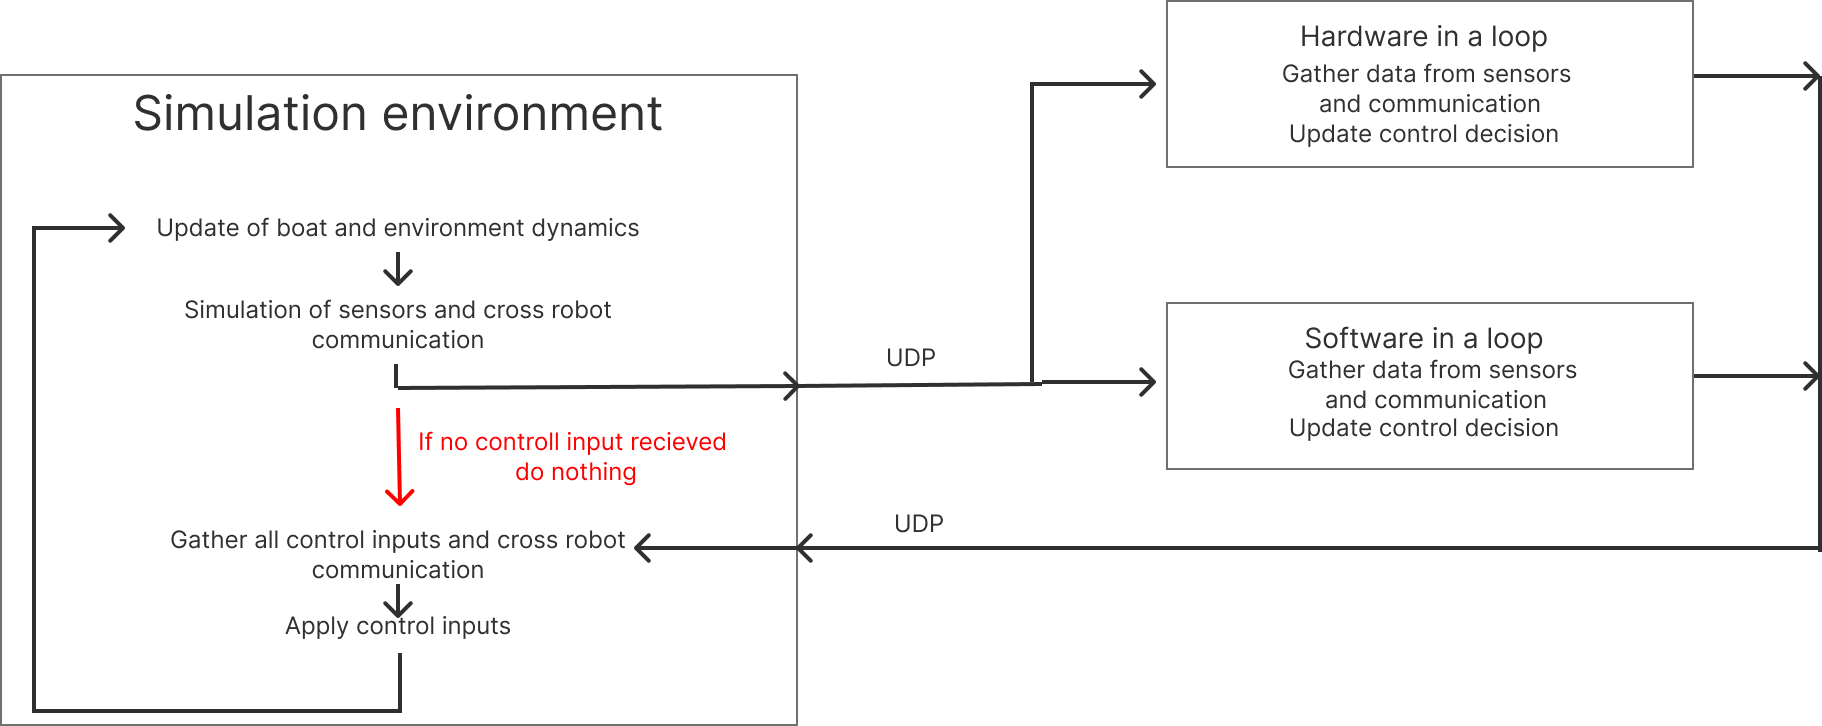
\includegraphics[width=0.7\textwidth]{images/simulation_schematic.png}
        
        {\small\textit{Proposed simulation dataflow.}}
      \end{center}

\end{abstract}
